\section{Задача протекания}
\subsection{Постановка задачи}

Для исходной системы зададим начальные условия, которые определяют задачу "протекания"

\begin{equation}
	\begin{cases}
		\begin{array}{l}
			\rho(0, x) = 1, x \in [0;10],\\
			u(0, x) = 0, x \in [0;10],\\
			u(t, 0) = \tilde{v}, t \in [0;T],\\
			\rho(t, 0) = \tilde{\rho}, t \in [0;T],\\			
			\frac{\partial u}{\partial x}(x) = 0, x=X, t \in [0;T]\\
		\end{array}
	\end{cases}
\end{equation}
Функции $f$ и $f_0$ примем равными нулю. $\tilde{\rho} \geqslant 1, \tilde{v} > 0 $. Суть эксперимента состоит в решении исходной задачи с введенными нами начальными значениями до момента стабилизации. Моментом стабилизации назовет время $T = N_0\tau$ при котором выполняется условие:
$$
||V^{N_0} - V^{N_0 - k}||_c < \varepsilon,
$$
$k \in 1,2,\dots$ - константа, $\varepsilon]$ подбирается опытным путем.

\subsection{Модификация разностной схемы}
Ввиду новых граничных условий, уравнения на $V$ и $H$ видоизменятся следующим образом:

Граничные условия на скорость и плотность при $m=0$:
$V_0^{n+1} = \tilde{u}$, $H_0^{n+1} = \tilde{\rho}$

Граничные условия на скорость при $m=M$:
$V_M^{n+1} = 0$, на $V_M^{n+1} - V_{M-1}^{n+1} = 0$

Граничные условия на плотность при $m=M$ ищутся чуть сложнее, необходимо учесть обнуление $\frac{\partial u}{\partial x}$ при $x=X$:\\

$
H_{t,M} + 0.5((V\hat{H})_{\bar{x},M} + H_MV_{\bar{x},M}) + 0.5h((HV)_{x\bar{x},M-1} - 0.5(HV)_{x\bar{x},M-2} + \\
+ H_M(V_{x\bar{x},M-1} - 0.5 V_{x\bar{x},M-2})) = 0
$\\

Примет вид: 
$
H_{t,M} + V_M\hat{H}_{\bar{x}, M} + 0.5h(V_M(H_{x\bar{x},M-1} - 0.5H_{x\bar{x},M-2}) - 0.5 V_{x\bar{x},M-2}) = 0
$\\

$
\frac{H_M^{n+1} - H_M^n}{\tau} + 0.5V_M^n\left(\frac{H_{M}^n-H_{M-1}^n}{h}\right) + \\
+ \frac{h}{2}\left(V_M\left(\frac{H_{M-2}^n-2H_{M-1}^n + H_{M}^n}{h^2} -\frac{1}{2}\frac{H_{M-3}^n-2H_{M-2}^n + H_{M-1}^n}{h^2}\right) -\frac{1}{2}\frac{V_{M-3}^n - 2V_{M-2}^n + V_{M-1}^n}{h^2}\right) = 0
$\\

$
H_M^{n+1}\left(\frac{1}{\tau} + \frac{V_M^n}{2h}\right) + H_{M-1}^{n+1}\left(-\frac{V_{M-1}^n}{2h}\right) = \frac{H_M^n}{\tau} - \\ \frac{h}{2}\left(V_M\left(\frac{H_{M-2}^n-2H_{M-1}^n + H_{M}^n}{h^2} -\frac{1}{2}\frac{H_{M-3}^n-2H_{M-2}^n + H_{M-1}^n}{h^2}\right) -\frac{1}{2}\frac{V_{M-3}^n - 2V_{M-2}^n + V_{M-1}^n}{h^2}\right)
$\\

\newpage
\subsection{Численные эксперименты}
В качестве измельчения сетки возьмем $\tau = 10^{-3} \, h = 10^{-2}$. Эксперементальным путем было подобрано значение $\varepsilon = 10^{-3}$, $k = 50$. Ввиду того, что при $C = 100$ и $\mu = 0.001$ сходимость схемы плохая, данные параметры не будем расссматривать при расчете различных вариантов начальных условий.


Далее приведены таблицы с временами стабилизации задачи.
\begin{center}
Table of stabilization time. $\mu = 0.1000$, $C = 10.0000$, $\gamma = 1.0000$
  
\begin{tabular}{|p{0.8in}|p{0.8in}|p{0.8in}|p{0.8in}|p{0.8in}|} \hline
$\tilde{\rho} / \tilde{v}$ &1 &2 &3 &4 \\ \hline 
1 &7.941e+00 &7.321e+00 &7.224e+00 &5.459e+00 \\ \hline 
2 &7.998e+01 &5.474e+01 &2.884e+01 &1.965e+00 \\ \hline 
3 &4.498e+02 &2.296e+02 &2.146e+01 &2.427e+00 \\ \hline 
4 &6.748e+02 &2.862e+02 &2.227e+01 &4.601e+00 \\ \hline 

\end{tabular}\\[20pt]
\end{center}

\begin{center}
Table of stabilization time. $\mu = 0.1000$, $C = 1.0000$, $\gamma = 1.0000$
  
\begin{tabular}{|p{0.8in}|p{0.8in}|p{0.8in}|p{0.8in}|p{0.8in}|} \hline
$\tilde{\rho} / \tilde{v}$ &1 &2 &3 &4 \\ \hline 
1 &1.108e+00 &2.641e+00 &1.011e+00 &6.187e+00 \\ \hline 
2 &7.427e+01 &1.577e+01 &7.542e+00 &4.883e+00 \\ \hline 
3 &6.437e+02 &1.297e+02 &6.615e+00 &4.420e+00 \\ \hline 
4 &6.962e+02 &1.163e+02 &6.126e+01 &4.178e+00 \\ \hline 

\end{tabular}\\[20pt]
\end{center}

\begin{center}
Table of stabilization time. $\mu = 0.1000$, $C = 1.0000$, $\gamma = 1.4000$
  
\begin{tabular}{|p{0.8in}|p{0.8in}|p{0.8in}|p{0.8in}|p{0.8in}|} \hline
$\tilde{\rho} / \tilde{v}$ &1 &2 &3 &4 \\ \hline 
1 &6.912e+00 &5.525e+01 &1.404e+01 &5.678e+00 \\ \hline 
2 &5.748e+01 &3.227e+01 &1.022e+01 &6.010e+00 \\ \hline 
3 &9.152e+01 &4.200e+01 &8.893e+00 &5.392e+00 \\ \hline 
4 &2.802e+02 &1.838e+02 &8.192e+01 &5.073e+00 \\ \hline 

\end{tabular}\\[20pt]
\end{center}


\newpage
\begin{center}
	Table of stabilization time. $\mu = 0.0100$, $C = 10.0000$, $\gamma = 1.0000$
	
	\begin{tabular}{|p{0.8in}|p{0.8in}|p{0.8in}|p{0.8in}|p{0.8in}|} \hline
		$\tilde{\rho} / \tilde{v}$ &1 &2 &3 &4 \\ \hline 
		1 &2.024e+01 &1.956e+01 &7.454e+01 &5.959e+01 \\ \hline 
		2 &2.948e+02 &5.477e+02 &9.254e+01 &3.825e+01 \\ \hline 
		3 &8.543e+02 &5.152e+02 &2.691e+02 &2.834e+01 \\ \hline 
		4 &1.691e+03 &7.695e+02 &7.146e+02 &1.669e+02 \\ \hline 
		
	\end{tabular}\\[20pt]
\end{center}

\begin{center}
	Table of stabilization time. $\mu = 0.0100$, $C = 1.0000$, $\gamma = 1.0000$
	
	\begin{tabular}{|p{0.8in}|p{0.8in}|p{0.8in}|p{0.8in}|p{0.8in}|} \hline
		$\tilde{\rho} / \tilde{v}$ &1 &2 &3 &4 \\ \hline 
		1 &8.719e+01 &2.613e+01 &8.054e+00 &9.112e+00 \\ \hline 
		2 &4.662e+02 &5.559e+01 &1.540e+01 &4.821e+01 \\ \hline 
		3 &7.068e+02 &2.279e+02 &2.583e+01 &4.235e+01 \\ \hline 
		4 &8.681e+02 &3.137e+02 &6.113e+01 &7.173e+01 \\ \hline 
		
	\end{tabular}\\[20pt]
\end{center}

\begin{center}
	Table of stabilization time. $\mu = 0.0100$, $C = 1.0000$, $\gamma = 1.4000$
	
	\begin{tabular}{|p{0.8in}|p{0.8in}|p{0.8in}|p{0.8in}|p{0.8in}|} \hline
		$\tilde{\rho} / \tilde{v}$ &1 &2 &3 &4 \\ \hline 
		1 &1.912e+02 &1.525e+02 &8.404e+01 &2.698e+01 \\ \hline 
		2 &3.228e+02 &1.227e+02 &7.022e+01 &1.110e+01 \\ \hline 
		3 &8.142e+02 &2.200e+02 &9.893e+01 &4.332e+01 \\ \hline 
		4 &1.512e+03 &3.336e+02 &1.153e+02 &7.073e+01 \\ \hline 
		
	\end{tabular}\\[20pt]
\end{center}


\newpage
Также приведем график значений функций $H$ и $V$ для разных временных слоев. $\tilde{\rho} = \tilde{u} = 1$

\begin{figure}[H]
	\centering
	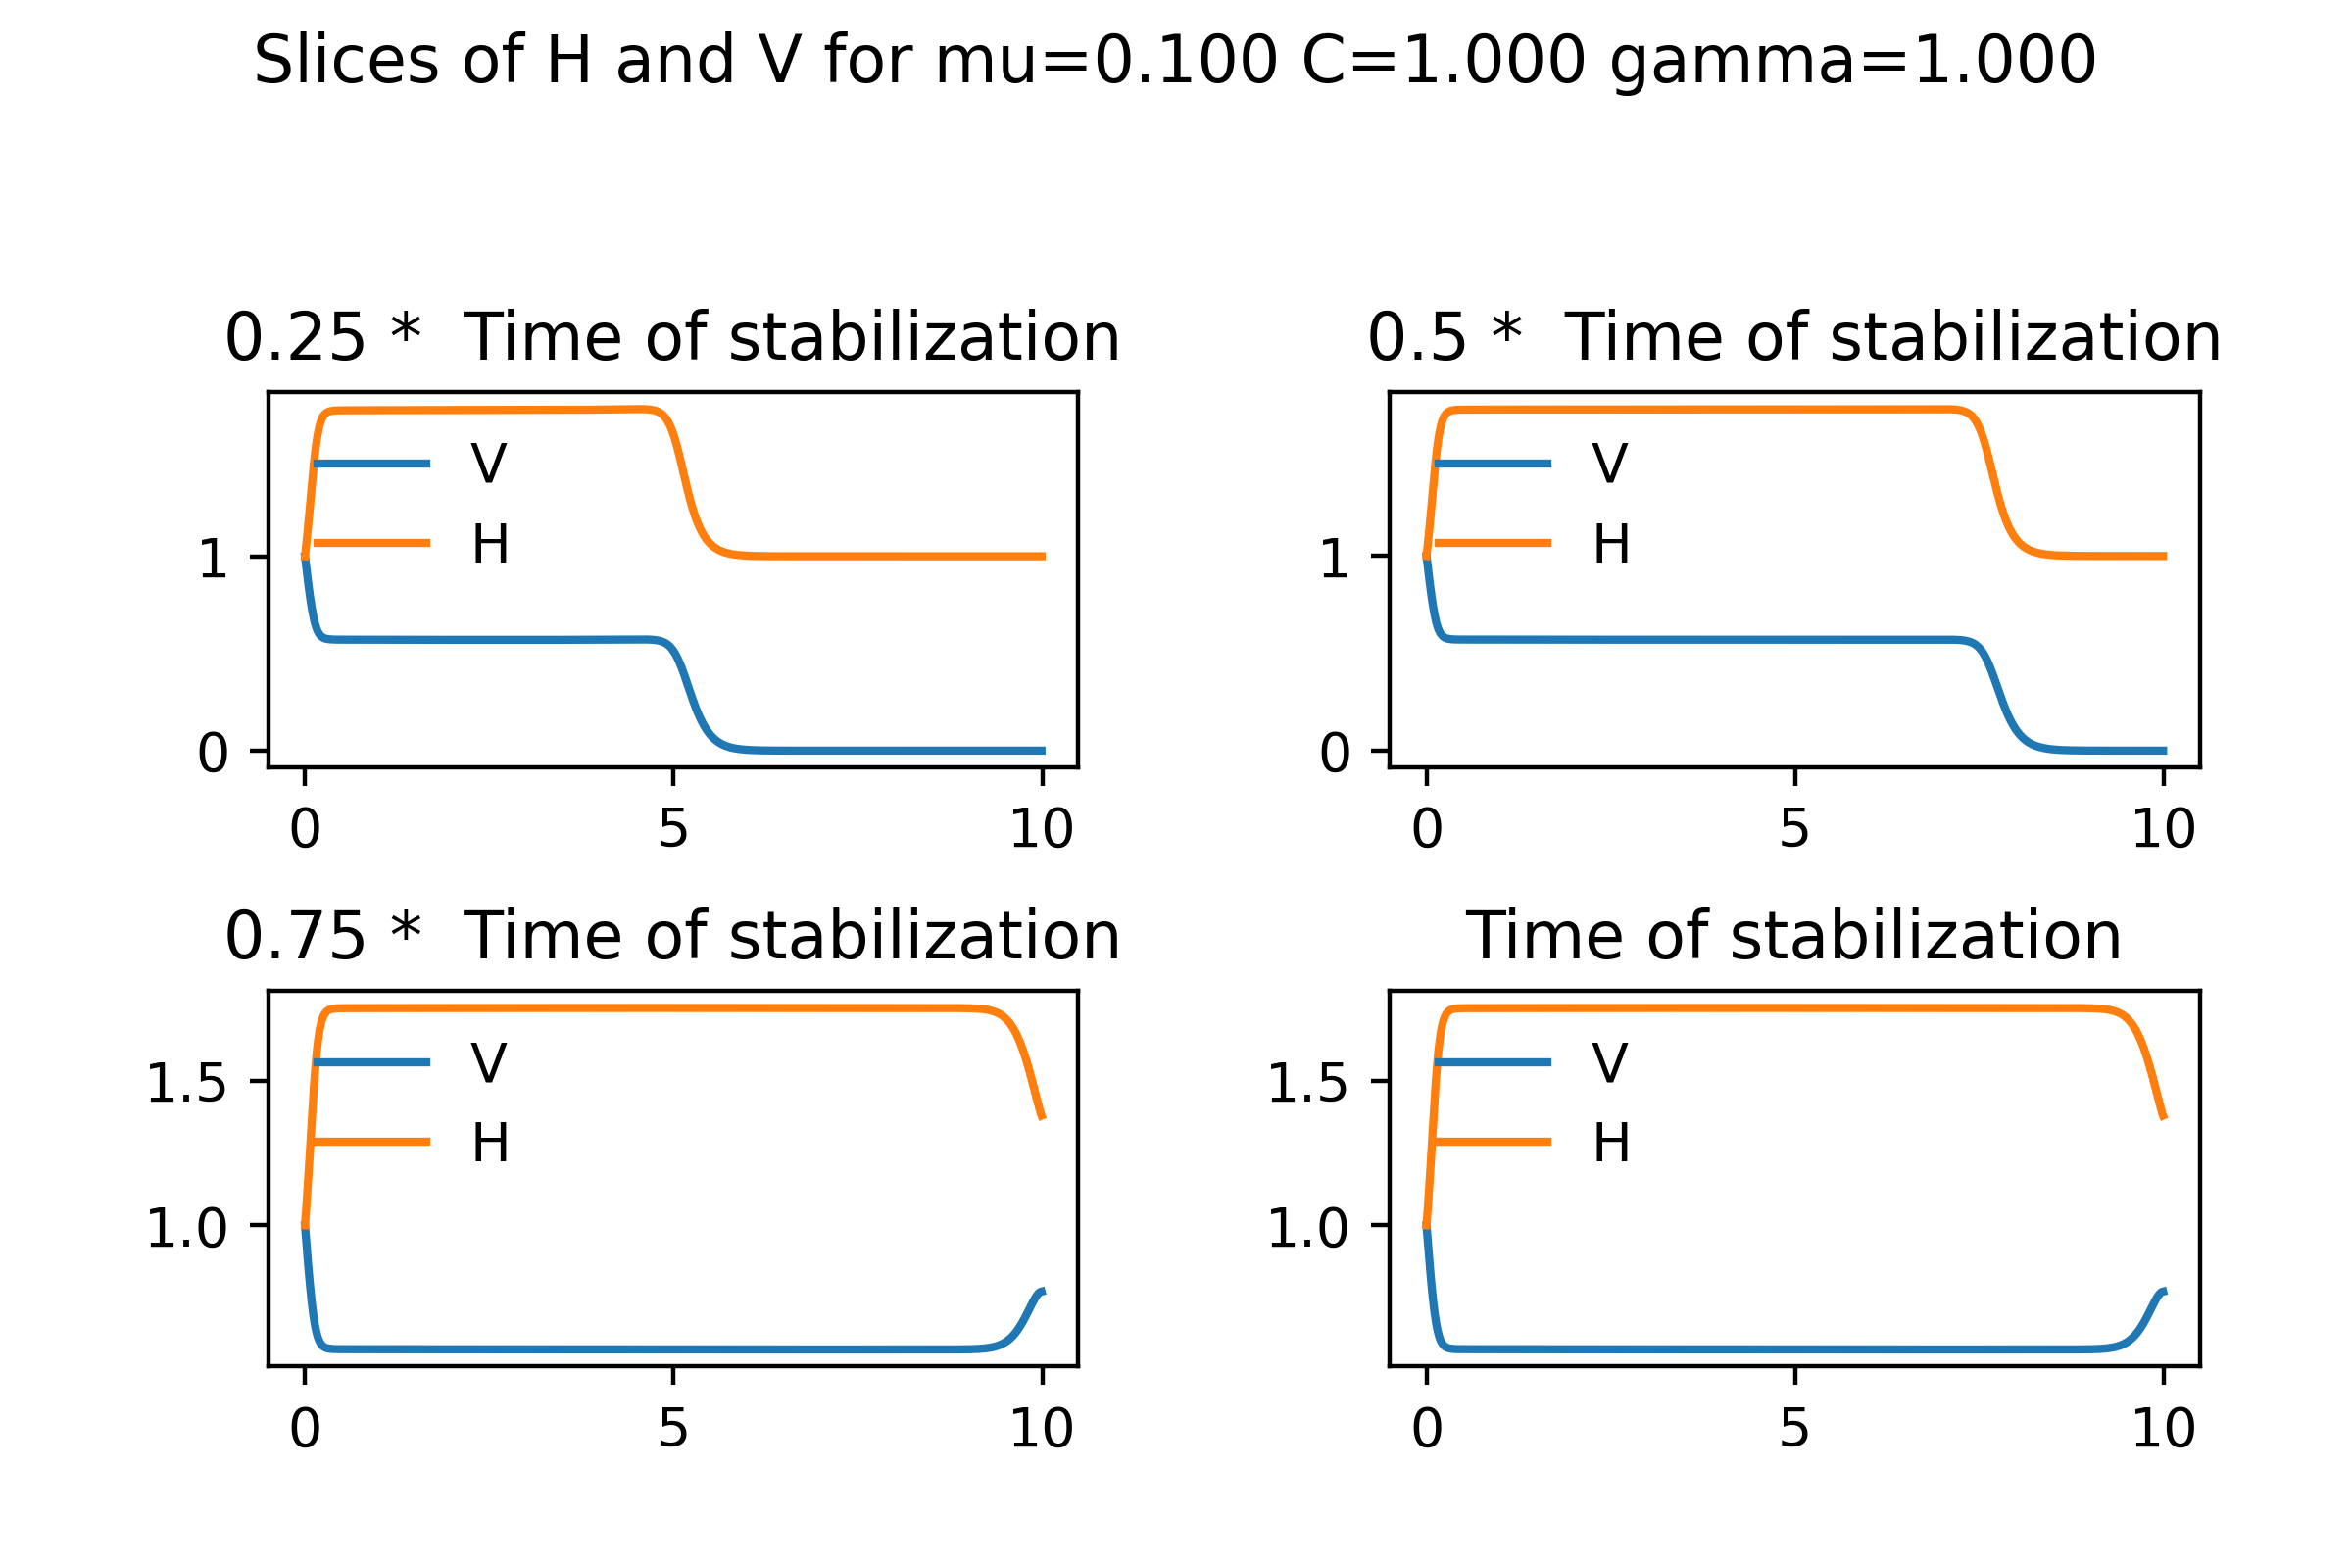
\includegraphics[scale=1.1]{../graph_data_flow/Slices_mu0.100_C1.000_gamma1.000.png}
\end{figure}


\subsection{Выводы}
При уменьшении $\mu$ время стабилизации значительно увеличивается. От $C$, $\gamma$ существенной зависимости не обнаружено, (небольшое увеличение времени стабилизации при $C=10$). При увеличении $\tilde{\rho}$ время стабилизации увеличивается, при увеличении $\tilde{u}$ время стабилизации уменьшается.

